%Created on: July 8, 2014       Edited by: Wesley Kyle
%Edited on:                     Edited by:
%Edited on:                     Edited by:
%Edited on:                     Edited by:
%Edited on:                     Edited by:
%Edited on:                     Edited by:
%Edited on:                     Edited by:
%Edited on:                     Edited by:


% This is a template for the production of all future lab documents
% 
% IMPORTANT: Edit only between the line "%%%start %%% DO NOT REMOVE THIS LINE"
% and %%%end %%% DO NOT REMOVE THIS LINE
%
% To compile the tex file use the command pdflatex

\documentclass[justified]{tufte-book}
\usepackage{graphicx} % allow embedded images
\setkeys{Gin}{width=\linewidth,totalheight=\textheight,keepaspectratio}
\usepackage{amsmath}  % extended mathematics
\usepackage{booktabs} % book-quality tables
\usepackage{units}    % non-stacked fractions and better unit spacing
\usepackage{multicol} % multiple column layout facilities
\usepackage{fancyvrb} % extended verbatim environments
\fvset{fontsize=\normalsize}% default font size for fancy-verbatim environments
\usepackage{tikz} %for drawing nice pictures
\usepackage{indentfirst}
\usepackage{enumitem}
\usepackage{fancyhdr}
\usepackage{soul}
\usepackage{marvosym}
\pagestyle{fancy}
\usepackage{float}
\allowdisplaybreaks % allows equations to span two pages if needed
\restylefloat{table}
\usetikzlibrary{arrows,snakes,shapes,calc,patterns}
\usetikzlibrary{circuits.ee.IEC}
%\usepackage[T1]{fontenc}
%\usepackage[utf8]{inputenc}

\fancyhf{} % clear all header and footer fields
\fancyfoot[C]{\footnotesize \thepage}
\renewcommand{\headrulewidth}{0pt}
\renewcommand{\footrulewidth}{0pt}


\begin{document}

\chapter{Vacuum Technology Laboratory - Companion Guide}


%%%start %%% DO NOT REMOVE THIS LINE

\section{Equipment and Setup}

\subsection{Part I: Mechanical Gauges and Pumps}

% first column
\begin{minipage}[t]{0.55\textwidth}
\begin{itemize}[noitemsep]
\item Hand operated vacuum pump
\item Edwards RV5 mechanical pump
\end{itemize}
\end{minipage}
%second column
\begin{minipage}[t]{0.45\textwidth}
\begin{itemize}[noitemsep]
\item Schematic diagram of vacuum pumping principles
\item 5 board-mounted gauges.
\end{itemize}
\end{minipage}

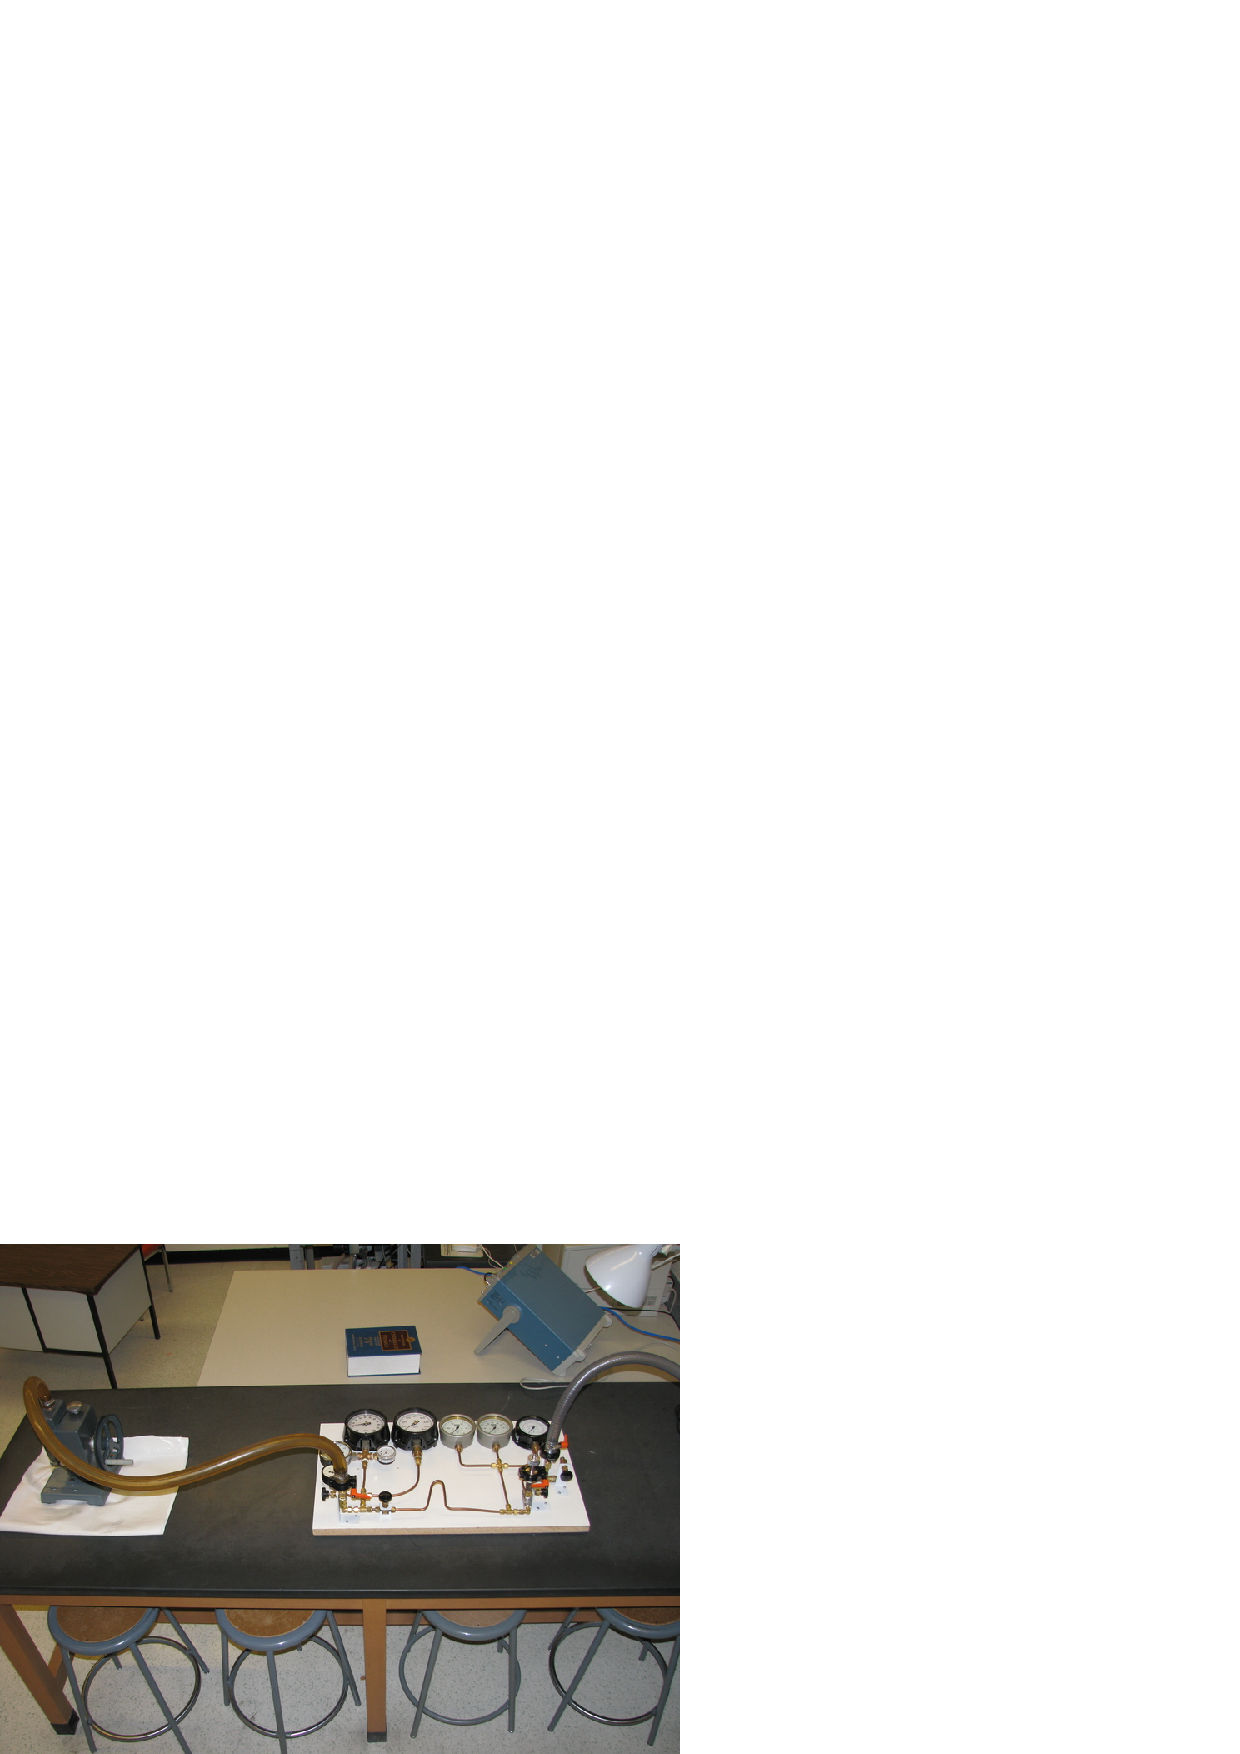
\includegraphics{Mechanical-Gauges-and-Pumps-Table8.pdf}
\caption{Part 1: Mechanical Gauges and Pumps Equipment Setup}
\label{pic:VACmec}
\end{figure}


II)   Sorption pump, liquid nitrogen and dewar, thermocouple vacuum gauge, safety glasses, heat gun.\newline
III)  "Leaky weld" assembly, Edwards RV5 mechanical pump, helium bottle with regulator and bench clamp, 2 labs stands, 2 fork clamps, 2 right-angle clamps.\newline
IV)   Vacuum manifold cart, Edwards RV5 mechanical pump, 2 anatek power supplies, connecting leads.\newline
V)    Edwards RV5 mechanical pump, foreline trap, 2 isolation valves, vacuum hose, 25cm tube with NW25 terminations, four-way cross with NW25 flanges, thermocouple vacuum guage, assortment of NW25 O-rings and metal centering rings. assortment of NW25 clamps, rubber gloves.\newline
VI)   Vernier capable computer, Vernier intrumentation amplifier, pumpdown_template.cmbl Loggerpro file, pumpdown and leakout curve apparatus, stopwatch.\newline
VII)  Diffstak equipment cart, RG-83 ionization guage controller, Edwards RV5 mechanical vacuum pump.
VIII) High Vacuum Turbo Molecular System.\newline
Components of vacuum system museum that match labels available in "label" section.\newline



Set up bench as shown in Figure \ref{pic:}.

\section{Maintenance}

\begin{enumerate}
\item 
\item 
\end{enumerate}

\section{Critical Points of Failure}

There are currently no known critical points of failure.

\section{Notes to the Instructor}
\begin{enumerate}
\item 
\item 
\item 
\end{enumerate}

\section{Prelab Questions}
\begin{enumerate}


\end{enumerate}


\section{Data Requirements}
\begin{enumerate}


\end{enumerate}


\section{Discussion}
\begin{enumerate}[resume]



\end{enumerate}




%%%end %%% DO NOT REMOVE THIS LINE

\end{document}
